%%%%%%%%%%%%%%%%%%%%%%%%%%%%%%%%%%%%%%%%%
% Structured General Purpose Assignment
% LaTeX Template
%
% This template has been downloaded from:
% http://www.latextemplates.com
%
% Original author:
% Ted Pavlic (http://www.tedpavlic.com)
%
% Note:
% The \lipsum[#] commands throughout this template generate dummy text
% to fill the template out. These commands should all be removed when 
% writing assignment content.
%
%%%%%%%%%%%%%%%%%%%%%%%%%%%%%%%%%%%%%%%%%

\documentclass{article}

\usepackage{fancyhdr} % Required for custom headers
\usepackage{lastpage} % Required to determine the last page for the footer
\usepackage{extramarks} % Required for headers and footers
\usepackage{graphicx} % Required to insert images
\usepackage[utf8]{inputenc}

% Margins
\topmargin=-0.45in
\evensidemargin=0in
\oddsidemargin=0in
\textwidth=6.5in
\textheight=9.0in
\headsep=0.25in 

\linespread{1.1} % Line spacing



\setlength\parindent{0pt} % Removes all indentation from paragraphs

%----------------------------------------------------------------------------------------
%	DOCUMENT STRUCTURE COMMANDS
%	Skip this unless you know what you're doing
%----------------------------------------------------------------------------------------

% Header and footer for when a page split occurs within a problem environment
\newcommand{\enterProblemHeader}[1]{
\nobreak\extramarks{#1}{#1 continued on next page\ldots}\nobreak
\nobreak\extramarks{#1 (continued)}{#1 continued on next page\ldots}\nobreak
}

% Header and footer for when a page split occurs between problem environments
\newcommand{\exitProblemHeader}[1]{
\nobreak\extramarks{#1 (continued)}{#1 continued on next page\ldots}\nobreak
\nobreak\extramarks{#1}{}\nobreak
}

\setcounter{secnumdepth}{0} % Removes default section numbers
\newcounter{homeworkProblemCounter} % Creates a counter to keep track of the number of problems

%----------------------------------------------------------------------------------------
%	NAME AND CLASS SECTION
%----------------------------------------------------------------------------------------

\newcommand{\lessonNumber}[1]{Lezione\ \##1} % Assignment title
\newcommand{\lessonDate}[4]{#1,\ #2\ #3\ #4} % Due date
\newcommand{\lessonCourse}[1]{#1} % Course/class
\newcommand{\lessonTime}[1]{#1} % Class/lecture time
\newcommand{\lessonTeacher}[1]{#1} % Teacher/lecturer
\newcommand{\lessonAuthor}[1]{#1} % Your name
\begin{document}

\section{Diagrammi delle attività (6)}

Aiutano a descrivere gli aspetti dinamici dei casi d'uso. Un'attività è un insieme di più azioni:
\begin{itemize}
	\item \textbf{Nodo iniziale:} da dove inizia l'esecuzione del processo;
	\item \textbf{Fork:} elaborazione che può essere anche parallela;
	\item \textbf{Join:} sincronizzazione tra più processi.
\end{itemize}


Il percorso che si descrive va dal nodo iniziale a quello finale ed è l'illustrazione di come l'attività deva essere eseguita. Ogni azione è descritta da un rettangolo con i bordi smussati e ha una descrizione interna. Una decisione, o \textbf{branch}, serve per modellare le condizioni (gli \textit{if}). La condizione si chiama \textbf{guardia}. L'insieme dei rami deve dare la totalità delle condizioni. Quando due o più branch si riuniscono abbiamo un \textbf{merge} che raggruppa il flusso.

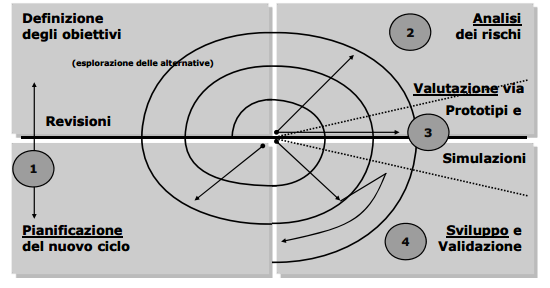
\includegraphics[width=0.5\columnwidth]{img5} % Example image

Questo diagramma mi permette di modellare anche il parallelismo. Questa fase parallela è detta \textbf{fork}. Il fork sdoppia un token in tante azioni che vengono eseguite in parallelo, o in sequenza se non ci interessa l'ordine di esecuzione dei rami. Per ricollegare più flussi paralleli usiamo la \textbf{join}, che potrebbe avere delle espressioni booleane che consentono di proseguire solo se queste sono soddisfatte.

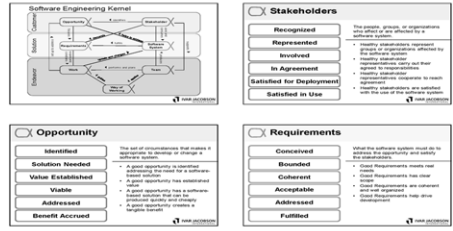
\includegraphics[width=0.75\columnwidth]{img6} % Example image

Può succedere che uno dei flussi, per qualche condizione, \textbf{muoia}, ovvero non abbia delle condizioni di terminazione. In questo caso non termina l'intera attività ma 
solo quel ramo.\\

Può esserci il caso in cui ho bisogno di definire delle \textbf{sottoattività} che saranno un'implementazione di un'azione (farla vedere al dettaglio). In un diagramma di attività, tra un'azione e un altro passo passano degli oggetti. Un'azione prende un oggetto in input e restituisce un oggetto in output.

\end{document}